% the va-template.tex file contains the document setup like styling
%%%%%%%%%%%%%%%%%%%%%%%%%%%%%%%%%%%%%%%%%%%%%%%%%%%%%%%%
% Example / Template for Zurich VA - Vertiefungsarbeit
%
% Based on:
%  Short Sectioned Assignment
%  http://www.LaTeXTemplates.com
%  Original author:
%  Frits Wenneker (http://www.howtotex.com)
%  License:
%  CC BY-NC-SA 3.0 (http://creativecommons.org/licenses/by-nc-sa/3.0/)
% ... and SOME hints, see URLs below
%%%%%%%%%%%%%%%%%%%%%%%%%%%%%%%%%%%%%%%%%
% plus
% https://github.com/psy-q/uol-msc-latex-template/blob/master/dissertation.tex
% PLUS
% tons of tiny tweaks, based on hints found on tex.stackexchange.com and others
% SEE BOTTOM OF THIS DOCUMENT FOR ALL HELPFUL LINKS THAT HELPED ME CREATING THIS.
% (Originally for https://twitter.com/LivUni ... but now simplified for this purpose)



%----------------------------------------------------------------------------------------
% BASIC PAGE SETUP

% A4 paper and 11pt font size
\documentclass[paper=a4, fontsize=12pt]{scrartcl}
\usepackage{geometry}   % borders e.g. [top=1.8cm, bottom=2.54cm, left=2.25cm, right=2.25cm]
\usepackage[utf8]{inputenc}
\usepackage{graphicx}  % use includegraphics to import jpegs
\usepackage[ngerman]{babel} % ngerman is neue deutsche rechtschreibung
\usepackage{pdfcomment} % permits inclusion of pdf comments (support in viewers varies)
\usepackage{amsmath,amsfonts,amsthm} % Math packages - to typeset mathematical formulas
\usepackage{lipsum}     % Used for inserting dummy 'Lorem ipsum' text into the template
\usepackage{sectsty}    % Allows customizing section commands
\usepackage{color}      % I have no idea
\usepackage{parskip}    % http://tex.stackexchange.com/questions/40429/how-to-use-the-parskip-package-space-in-between-paragraphs

% definition of custom color NAMES for later use - provide their RGB values here
\usepackage[usenames,dvipsnames,svgnames,table]{xcolor}
\definecolor{listingBgColor}{rgb}{1,1,1}
\definecolor{UOLBlue}{rgb}{0,0.03,0.25}
\definecolor{DarkBlue}{rgb}{0.05,0.05,0.35}
\definecolor{DarkRed}{rgb}{0.45,0.03,0.2}
\definecolor{LightGray}{rgb}{0.97,0.97,0.97}

% http://stackoverflow.com/questions/1012799/latex-prevent-line-break-in-a-span-of-text
\def\myurl{\hfil\penalty 100 \hfilneg \hbox}

% drawing sequence diagrams - google tikz uml and yes, UML sequence diagrams ;)
% \usepackage{tikz} % \usepackage{tikz-uml} % \usepackage{pgf-umlsd} %
% \usepgflibrary{arrows} % for pgf-umlsd

%% OUTLINE configuration.
%% Only here as howto should you wish to TYPSET your outline.
%% Use this if you are requested to SUBMIT such outline. Otherwise draft it.
%% http://tex.stackexchange.com/questions/12279/outline-of-style-i-a-i-a-1
%% adjusted to match https://owl.english.purdue.edu/owl/resource/544/03
\usepackage{outlines}
\usepackage{enumitem}
%% See outlines latex package docs if needed - you can control numbering per depth/level
\setenumerate[1]{label=\Roman*.}
\setenumerate[2]{label=\Alph*.}
\setenumerate[3]{label=\arabic*.}
\setenumerate[4]{label=\alph*.}

%% HTTP / Web-Links formatting
%\usepackage{url}  % This makes \url work
%\urlstyle{same}   % http://tex.stackexchange.com/questions/667/typeset-url-in-a-non-typewriter-font
\usepackage[]{hyperref}
\hypersetup{
    backref=false,
    colorlinks=true,
    citecolor=gray,
    linkcolor=gray,
    urlcolor=gray,
}
% \usepackage[hidelinks]{hyperref}

%----------------------------------------------------------------------------------------
% Source code listings
% \begin{lstlisting}[language=html] .... \end{lstlisting}
% https://en.wikibooks.org/wiki/LaTeX/Source_Code_Listings
\usepackage{listings}
\usepackage{textcomp}
\lstset{
    backgroundcolor=\color{listingBgColor},
    tabsize=2,
    rulecolor=\color[rgb]{0.1,0.1,0.1},
    numberstyle=\tiny\color{black},
    upquote=true,
    aboveskip={1.5\baselineskip},
    columns=fixed,
    showstringspaces=false,
    extendedchars=true,
    breaklines=true,
    prebreak = \raisebox{0ex}[0ex][0ex]{\ensuremath{\hookleftarrow}},
    frame=single,
    showtabs=false,
    showspaces=false,
    keepspaces=true,
    showstringspaces=false,
    identifierstyle=\ttfamily,
    %basicstyle=\scriptsize,
    %captionpos=b, % caption position; b for bottom; default top
    basicstyle=\footnotesize\ttfamily,
    keywordstyle=\color[rgb]{0,0,1},
    commentstyle=\color[rgb]{0.133,0.545,0.133},
    stringstyle=\color[rgb]{0.627,0.126,0.941},
}

% for pseudo code -- https://en.wikibooks.org/wiki/LaTeX/Algorithms
\usepackage{algorithmicx}
\usepackage{algpseudocode}
\usepackage{algorithm}

% allow manual caption/figure numbering
% http://tex.stackexchange.com/questions/199207/no-caption-number-for-figures-and-tables
\usepackage{caption}

% side-by-side pictures
% http://tex.stackexchange.com/questions/37581/latex-figures-side-by-side
\usepackage{subcaption}

% hierarchical diagrams using forest
% http://tex.stackexchange.com/questions/191001/how-to-draw-a-hierarchical-diagram-in-tikz
% \usepackage{forest}
% \usetikzlibrary{arrows.meta, shapes.geometric, calc, shadows}
% \colorlet{mygreen}{green!75!black}

%%% USE-CASE DESCRIPTIONS (UML / UML2)
%%% http://tex.stackexchange.com/questions/10293/latex-template-for-use-cases

% \usepackage{booktabs} % ???

%----------------------------------------------------------------------------------------
% tweakable style: header colors, document font (uncomment for Arial-Like)

% colorize headers?
%\chapterfont{\color{LightGray}}  % sets colour of chapters
%\sectionfont{\color{DarkRed}}
%\setkomafont{disposition}{\color{UOLBlue}\bfseries}

% Document Font - UoL Master Thesis requires sans serif
%\renewcommand{\familydefault}{\sfdefault}
%\usepackage{helvet}

%----------------------------------------------------------------------------------------
% Bibliography settings - The list of references / citations

\usepackage{fourier} % Use the Adobe Utopia font for the document

%%% BIBER works with your .bib files to include bibliography in final doc
%%% There are TONS of citation styles (almost per university)
%%% For HOMEWORK-like stuff, select one you like ;) - Generic teachers know ONE if any.
\usepackage[
    backend=biber,
    style=authoryear,%-ibid,
    dashed=false, % re-print recurring author names in bibliography
    citestyle=authoryear,
    %bibstyle=apalike,
    sortcites=false,
    block=space,
    useprefix=true, % de.. http://tex.stackexchange.com/questions/134258/harvard-style-bibliography-with-biblatex-almost-but-not-quite
    sortlocale=de_DE,
    natbib=true,
    url=true,
    maxcitenames=3,
    maxbibnames=99,  % show all authors in bib (not "et al") #SaneDefaults ?!
    firstinits=true, % use initials in bibliography
    uniquename=false, % http://tex.stackexchange.com/questions/65747/citation-style-in-biblatex-1-get-rid-of-first-names-2-remove-comma-before
    uniquelist=false,
    doi=true,
    eprint=false
]{biblatex}
%% The name of the file that contains all our refrences (separately. So we just reference them in this file.)
\addbibresource{va-bibliography.bib}

\renewcommand*{\finalandcomma}{} %% do not put comma before final author's "and" / "&" #SaneDefaults
% http://tex.stackexchange.com/questions/1554/biblatex-displaying-all-authors-of-multi-author-works-in-the-bibliography

% attach files to pdfs -- http://tex.stackexchange.com/questions/94811/attaching-file-into-a-pdf-with-pdflatex-will-crash-adobe-reader
% For including our malware payload. Try Eicar ;) Then submit to TurnitIn. Do not use real malware please.
\usepackage{attachfile}

% http://tex.stackexchange.com/questions/76262/biblatex-format-for-online-sources


%----------------------------------------------------------------------------------------
% tweak headers style and numbering

\usepackage{fancyhdr} % Custom headers and footers
\pagestyle{fancyplain} % Makes all pages in the document conform to the custom headers and footers
%\fancyhead{} % No page header - if you want one, create it in the same way as the footers below
\fancyhead[L]{Vertiefungsarbeit}
\fancyhead[C]{PM-99999}
\fancyhead[R]{Beispiel-Vorlage VA}

\fancyfoot[L]{Donald Duck} % Empty left footer
\fancyfoot[C]{} % Empty center footer
\fancyfoot[R]{\thepage} % Page numbering for right footer
\renewcommand{\headrulewidth}{0pt} % Remove header underlines
\renewcommand{\footrulewidth}{0pt} % Remove footer underlines
\setlength{\headheight}{13.6pt} % Customize the height of the header
\numberwithin{equation}{section} % Number equations within sections (i.e. 1.1, 1.2, 2.1, 2.2 instead of 1, 2, 3, 4)
%\numberwithin{figure}{section} % Number figures within sections (i.e. 1.1, 1.2, 2.1, 2.2 instead of 1, 2, 3, 4)
\numberwithin{table}{section} % Number tables within sections (i.e. 1.1, 1.2, 2.1, 2.2 instead of 1, 2, 3, 4)
\setlength\parindent{0pt} % Removes all indentation from paragraphs - comment this line for an assignment with lots of text

% Quotations. Zitate. Also nicht Referenzen/Verweise auf andere Literatur, sondern ein 1:1 Auszug aus einem fremden Werk.
\usepackage{epigraph}
% https://www.sharelatex.com/learn/Typesetting_quotations
% Example usage:
% \epigraph{All human things are subject to decay, and when fate summons, Monarchs must obey}{\textit{Mac Flecknoe \\ John Dryden}}

%----------------------------------------------------------------------------------------
%	TITLE SECTION

% Create horizontal rule command with 1 argument of height
\newcommand{\horrule}[1]{\rule{\linewidth}{#1}}

% Your university, school and/or department name(s)
\title{
    \normalfont \normalsize
    \textsc{Stadt Zürich} \\ [25pt]
    \horrule{0.5pt} \\[0.4cm] % Thin top horizontal rule
    \huge Beispiel-Vorlage für eine Vertiefungsarbeit \\ % The assignment title (to be defined per doc)
    \horrule{2pt} \\[0.5cm] % Thick bottom horizontal rule
}

% Mail/Link author?
\author{Donald Duck}

% Today's date or a custom date
\date{\normalsize\today}
% To date back a assignment (re-submission or whatever):
% \date{Sunday 18\textsuperscript{th} January, 2016}


% allow multi-line comments using \begin{comment} ... \end{comment}
% Imagine you could do this in Python ;) Or Perl?
\usepackage{verbatim}


% LINKS THAT MADE THIS HAPPEN

% look into standard.bbx
% http://tex.stackexchange.com/questions/176297/automatically-highlight-undefined-references
% http://tex.stackexchange.com/questions/8351/what-do-makeatletter-and-makeatother-do
% https://www.ctan.org/pkg/csquotes?lang=en --- consider use?
% http://tex.stackexchange.com/questions/180986/biblatex-no-period-after-book-and-collection-titles
% http://www.khirevich.com/latex/biblatex/
% http://tex.stackexchange.com/questions/12806/guidelines-for-customizing-biblatex-styles
% http://tex.stackexchange.com/questions/1492/passing-parameters-to-a-document
% http://tex.stackexchange.com/questions/3730/using-harvard-referencing-style
% http://tex.stackexchange.com/questions/102937/natbib-use-the-harvard-referencing-system
% http://tex.stackexchange.com/questions/26516/how-to-use-biber
% http://tex.stackexchange.com/questions/102662/harvard-reference-using-biblatex
% https://www.sharelatex.com/learn/Biblatex_citation_styles
% https://www.overleaf.com/latex/examples/a-simple-example-showing-how-to-create-harvard-style-referencing-in-latex/mnwzgkyvdbyy#.Vi6PoeorLdQ
% https://www.sharelatex.com/learn/Bibtex_bibliography_styles
% http://tex.stackexchange.com/questions/134258/harvard-style-bibliography-with-biblatex-almost-but-not-quite
% http://tex.stackexchange.com/questions/2095/simplest-way-to-typeset-entire-document-in-sans-serif-helvetica
% http://www.tug.dk/FontCatalogue/

% EOF

% ---- Your work below --------------------------------------------

\begin{document}
\maketitle % Print the title
\thispagestyle{empty}
\newpage
\tableofcontents
\thispagestyle{empty}
\newpage

\section{Einleitung}
\lipsum[1] % REPLACE WITH YOUR TEXT

\section{Allgemein Wissenswertes zum Thema X}
\lipsum[2-4] % REPLACE WITH YOUR TEXT

\section{Nebenaspekte und Schauplätze / Previous work}
\lipsum[5-6] % REPLACE WITH YOUR TEXT

\section{Meine STORY}
\lipsum[7-8] % REPLACE WITH YOUR TEXT
Here's an example outline:
\begin{outline}[enumerate]
  \1 Introduction
  \1 Background
  \1 First major point
    \2 subs if any
  \1 Second and further points
  \1 Opposing views
    \2 ack em
    \2 provide response
  \1 Conclusion
    \2 restate thesis
    \2 recommended steps
    \2 why important
\end{outline}
\lipsum[9-11] % REPLACE WITH YOUR TEXT
\paragraph{Source code} can be set using using \verb|\begin{lstlisting}[language=bash]| ...
  \begin{lstlisting}[language=bash]
  FOO="bar baz"
  echo ${FOO}
  \end{lstlisting}
  % Include source from file:
  % \lstinputlisting{../FooBar.cpp}

  or set using a default verbatim environment ...
  \begin{verbatim}
  FOO="bar baz"
  echo ${FOO}
  \end{verbatim}

\section{Weitere Tätigkeiten, gesammelte Erkenntnisse}
	\lipsum[12] % REPLACE WITH YOUR TEXT

	\subsection{A subsection}
	  Foo bar baz ``bli bla blu'' blip bing bong, use \verb|\citep{...bibref...}| for citations
	  using parantheses like \citep{DBLP:books/aw/Knuth73}.
	  \textbf{Bold font} can be set using \verb|\textbf{...}|.
	  For in-text-citations, to name an author like \textcite{DBLP:books/aw/Knuth73},
	  use \verb|\textcite{...bibref...}|. Ever wanted to
	  write \texttt{rm -rf /}? Do it using \verb|\texttt{...}| for normal text
	  or using \verb!\verb|...|! for \LaTeX\ commands. Enforce line breaks
	  using double back slashes like here.
	  \\
	  Use \verb|\textcolor{colorname}{text...}|
	  to write for example in \textcolor{blue}{something} color.
	  \\
	  \textit{Italic Text}: Use \verb|\textit{...}|.
	  Good old \textsc{Kapitälchen} - what for? Emphasize using \verb|\emph{...}|: \emph{it is important}!
	  Does \citeauthor{DBLP:books/aw/Knuth73}'s quote inspire you?
	  \\
	  Use \verb|\citeauthor{...bibref...}|.
	  \texttt{citep} creates same as \texttt{parencite}: \citep{DBLP:books/aw/Knuth73}.
	  \lipsum[13] % REPLACE WITH YOUR TEXT

  	\subsection{Another subsection}
    	\lipsum[1] % REPLACE WITH YOUR TEXT

\section{Ausklang mit Medien - Fotos, Statistiken, Gerichte...}
\lipsum[14] % REPLACE WITH YOUR TEXT
\begin{figure}[H]
	\centering
	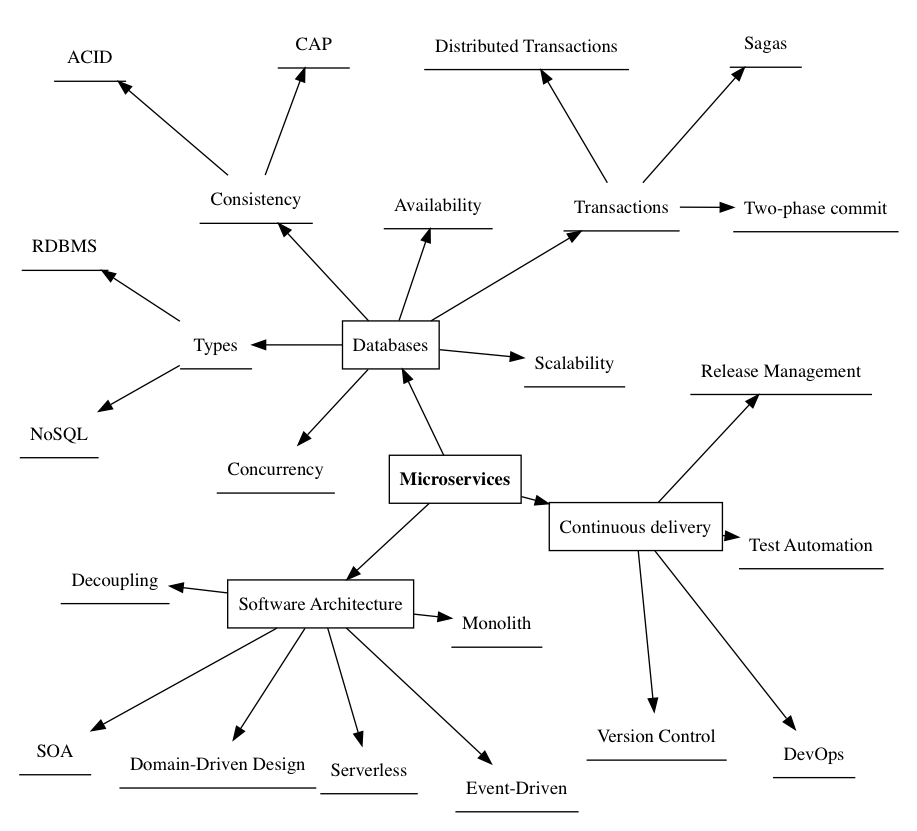
\includegraphics[width=70mm]{relevance-tree_map-mindmap.png}
	\caption{This is an example mindmap or relevance tree, created using dotty from GraphViz}
\end{figure}
\lipsum[15-17] % REPLACE WITH YOUR TEXT
Two images side by side example ... May come in handy.
\begin{figure}[H]
	\centering
	\begin{subfigure}{.5\textwidth}
	  \centering
	  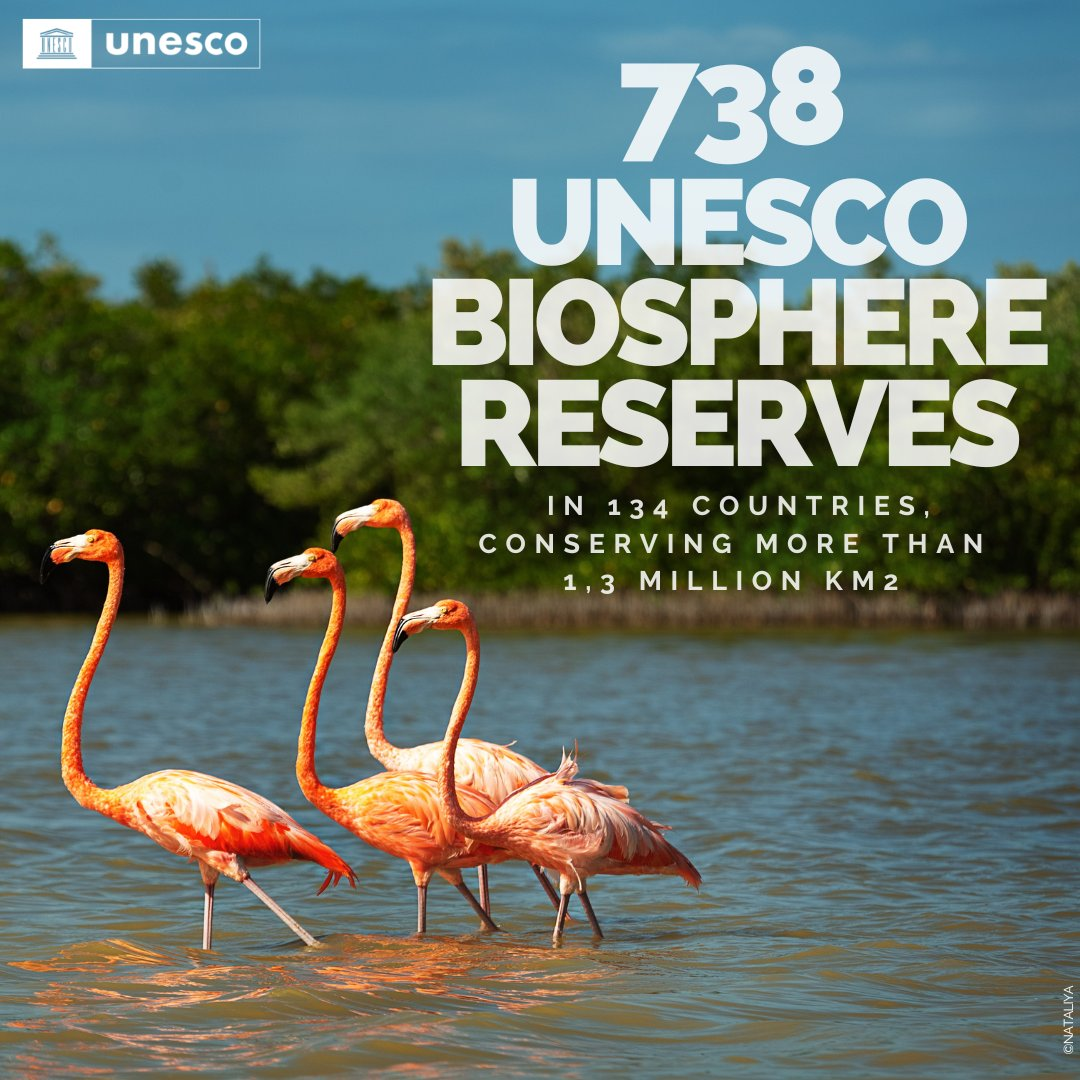
\includegraphics[width=.9\linewidth]{example-unesco.jpg}
	  \caption{UNESCO example 1}
	  \label{fig:sub1}
	\end{subfigure}%
	\begin{subfigure}{.5\textwidth}
	  \centering
	  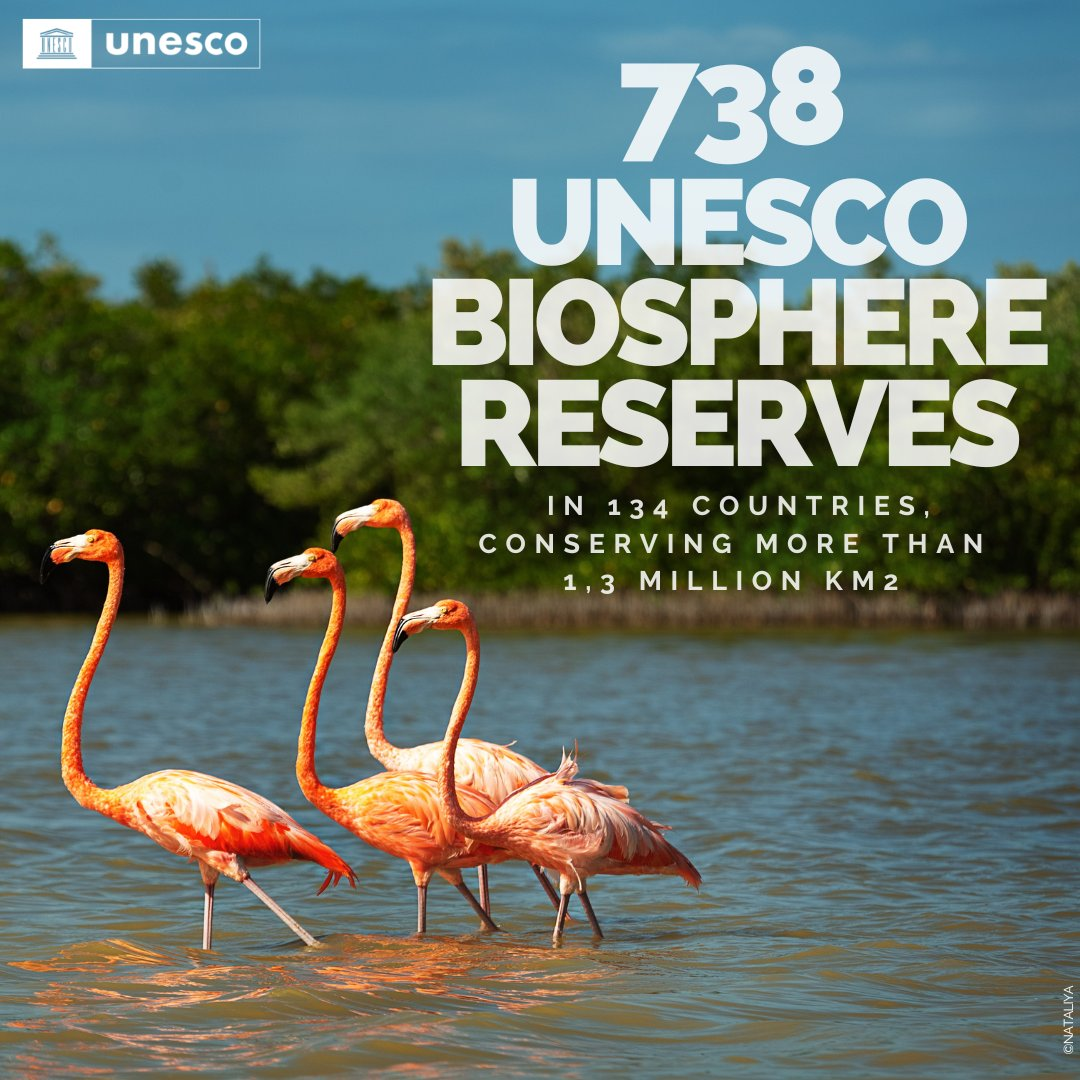
\includegraphics[width=.9\linewidth]{example-unesco.jpg}
	  \caption{Same image for illustration}
	  \label{fig:sub2}
	\end{subfigure}
	\caption{See, two images side by side. Cool?!}
	\label{fig:test}
\end{figure}


\section{Schlusswort - Conclusions}
\lipsum[18] % REPLACE WITH YOUR TEXT
Look, we know this\citep{DBLP:books/aw/Knuth73} and that.
And as Knuth told us before\citep{DBLP:books/daglib/0030428},
we have proof for facts\citep{DBLP:journals/cacm/KnuthS21}.

\section{Persönlicher Rückblick - Ausblick (``future work'')}
\lipsum[19] % REPLACE WITH YOUR TEXT


%% The rest is called Appendix and numbered as such, usually
%% https://latex-tutorial.com/latex-appendix/
\appendix

\section{Arbeitstagebuch - Diary of work}
FYI - Taken from \url{https://en.wikibooks.org/wiki/LaTeX/Tables}

\begin{tabular}{ | l | l | l | p{5cm} |}
  \hline
  Day & Min Temp & Max Temp & Summary \\ \hline
  Monday & 11C & 22C & A clear day with lots of sunshine.
  However, the strong breeze will bring down the temperatures. \\ \hline
  Tuesday & 9C & 19C & Cloudy with rain, across many northern regions. Clear spells
  across most of Scotland and Northern Ireland,
  but rain reaching the far northwest. \\ \hline
  Wednesday & 10C & 21C & Rain will still linger for the morning.
  Conditions will improve by early afternoon and continue
  throughout the evening. \\
  \hline
\end{tabular}

\section{Literaturverzeichnis}
\printbibliography % This will insert the BIBER magic here #References #Citationns

\section{Abbildungsverzeichnis} % Remind me to complete this #FIXME :)
%\thispagestyle{empty}
\listoffigures
% \listoftables - Overview of all TABLES

\section{Projektbeschreibung}
\lipsum[11] % REPLACE WITH YOUR TEXT



\end{document}
